\chapter{Teorema de Liouville y flujo hamiltoniano}

\lectureoverview{Las ecuaciones de Hamilton hacen más que reformular las ecuaciones del movimiento. Definen un campo de velocidades en el espacio de fases cuya divergencia se anula. Esa sencilla cancelación es el teorema de Liouville: la evolución hamiltoniana conserva el volumen del espacio de fases. Llegaremos a él siguiendo el orden en que su significado se hace visible---: primero, la conservación de la energía; luego, las superficies de energía constante; después, un fluido de posibles condiciones iniciales; y, por último, el contraste entre un flujo que conserva el volumen y un sumidero disipativo. El mismo lenguaje conduce de forma natural a los corchetes de Poisson.}

\section{¿Por qué otra formulación de la mecánica?}

El teorema que buscamos es la contraparte clásica continua de los diagramas de estados reversibles que presentamos al comienzo del curso. En una ley discreta reversible, cada estado tiene una flecha que entra y otra que sale. El presente basta para determinar tanto el estado siguiente como el anterior. Una ley defectuosa envía muchos estados a un mismo sumidero: puede determinar el futuro, pero ya no permite reconstruir el pasado.

El teorema de Liouville describe qué ocurre con esa distinción cuando el conjunto de estados es un espacio de fases continuo. La expresión que sustituye a «una flecha que entra y otra que sale» será \emph{tanto flujo de entrada como de salida}. Sin embargo, antes de darle un sentido matemático a esa expresión, debemos reconstruir el flujo a partir de las ecuaciones de Hamilton.

Al hacerlo, nos encontramos con una paradoja histórica. Hamilton, Jacobi, Lagrange y Poisson elaboraron formulaciones complejas y hermosas de la mecánica clásica sin conocer la teoría cuántica, en la que esas formulaciones llegarían a ser indispensables. Newton tenía un objetivo directo: el movimiento de los planetas. Lagrange y Hamilton también se ocuparon de problemas físicos, pero exploraron analogías y estructuras que iban mucho más allá de una órbita concreta. La acción estacionaria en mecánica se parecía a los principios del tiempo mínimo en óptica; el movimiento de los rayos y el de las partículas podían expresarse en formas matemáticas paralelas. Simplificaron, reorganizaron y unificaron las ecuaciones porque las propias estructuras parecían contener física.

Ahora sabemos que ese instinto fue extraordinariamente fecundo. Desde el punto de vista lógico, muchas características de la mecánica clásica pueden entenderse como límites de la mecánica cuántica. Históricamente, el orden fue inverso: primero se descubrieron las estructuras clásicas y solo mucho después se comprendió su uso más profundo. Una provocadora broma atribuida a Feynman señalaba esta idea al contrastar las matemáticas desarrolladas desde dentro con la física, limitada por un interlocutor externo: el mundo físico. La broma no es un argumento, pero la distinción es útil: aquí la belleza formal importa porque la naturaleza recurre una y otra vez a estas estructuras formales.

\begin{classroomqa}
  \audiencequestion{¿Tenía Newton el concepto moderno de energía cinética y dónde se originó el concepto de energía?
  \lecturetimestamp{00:04:24--00:05:50}}
  \lecturerresponse{La mecánica de Newton se organizaba en torno a la fuerza y el movimiento, no a un principio general de energía plenamente desarrollado. En esta discusión no se establece con certeza quién tuvo prioridad histórica. La \emph{vis viva} de Leibniz, \(\sum_i m_i v_i^2\), fue una precursora importante y equivale al doble de la energía cinética moderna. Más adelante, los estudios sobre el calor situaron en primer plano la conversión entre calor y trabajo mecánico. Las primeras teorías del calórico trataban el calor como una sustancia conservada, por lo que la idea moderna de formas de energía intercambiables surgió gradualmente.}
\end{classroomqa}

\section{Ecuaciones de Hamilton y conservación de la energía}

Sea un sistema con \(n\) pares canónicos,
\begin{equation}
  (q_i,p_i),\qquad i=1,\ldots,n.
  \label{eq:l7-canonical-pairs}
\end{equation}
Hay un momento por cada coordenada y una coordenada por cada momento. La ley del movimiento se expresa mediante una sola función,
\begin{equation}
  H=H(q_1,\ldots,q_n,p_1,\ldots,p_n,t),
  \label{eq:l7-hamiltonian}
\end{equation}
y las ecuaciones de Hamilton son
\begin{equation}
  \boxed{
  \dot q_i=\frac{\partial H}{\partial p_i},
  \qquad
  \dot p_i=-\frac{\partial H}{\partial q_i}.}
  \label{eq:l7-hamilton-equations}
\end{equation}
El signo forma parte de la estructura canónica. La ecuación de \(q\) lleva el signo más; la ecuación de \(p\), el signo menos.

\begin{figure}[htbp]
  \centering
  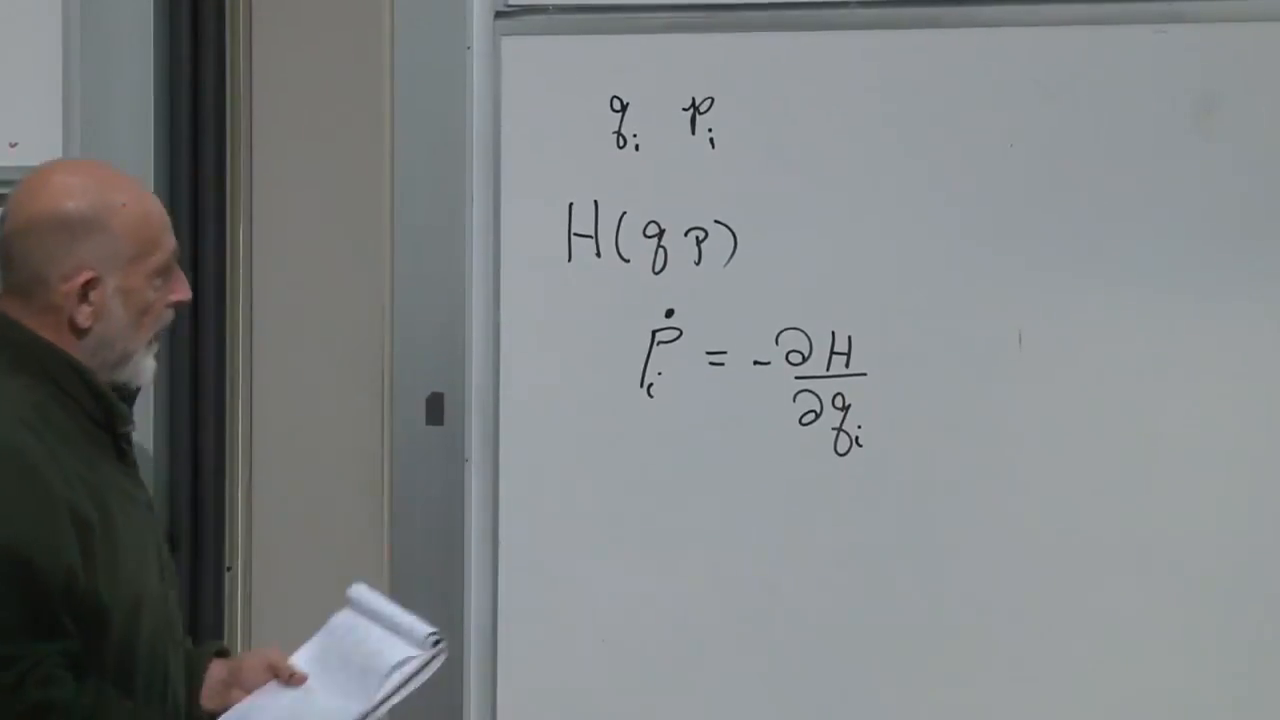
\includegraphics[width=0.82\textwidth]{lecture_07_figure_02.png}
  \caption{Variables canónicas, la función \(H(q,p)\) y la ecuación de Hamilton para el momento al comienzo del repaso.}
  \lectureframe{00:07:29}
\end{figure}

Aunque las ecuaciones aparecen en pares indexados, la dinámica no tiene por qué separarse par por par. El hamiltoniano puede acoplar todos los \(q_i\) y \(p_i\), de modo que \(\dot p_1\), por ejemplo, puede depender del estado de todo el sistema.

\begin{classroomqa}
  \audiencequestion{¿Es ahora axiomática la presentación? ¿Qué relación entre \(p\) y \(q\) se ha supuesto?
  \lecturetimestamp{00:17:08--00:18:18}}
  \lecturerresponse{Las ecuaciones de Hamilton definen la teoría formal una vez especificados \(H(q,p)\) y los pares canónicos. No hay una hipótesis adicional universal \(p=m\dot q\). Esa relación se cumple para una partícula cartesiana ordinaria con energía cinética cuadrática, pero otras coordenadas y otros hamiltonianos dan otras relaciones entre el momento-- y la velocidad. Las propias ecuaciones proporcionan la relación mediante \(\dot q_i=\partial H/\partial p_i\). Determinar si un hamiltoniano propuesto se realiza en la naturaleza es una cuestión física adicional.}
\end{classroomqa}

Ahora podemos recuperar la conservación de la energía con un solo razonamiento. A lo largo de una trayectoria, la derivada total de \(H\) es
\begin{equation}
  \frac{dH}{dt}
  =
  \sum_i\left(
    \frac{\partial H}{\partial q_i}\dot q_i
    +\frac{\partial H}{\partial p_i}\dot p_i
  \right)
  +\frac{\partial H}{\partial t}.
  \label{eq:l7-total-h-derivative}
\end{equation}
El último término representa la dependencia explícita del tiempo a \(q\) y \(p\) fijos, quizá porque está cambiando un parámetro prescrito externamente. Sustituyendo la ec.~\eqref{eq:l7-hamilton-equations},
\begin{align}
  \frac{dH}{dt}
  &=
  \sum_i\left[
    \frac{\partial H}{\partial q_i}
    \frac{\partial H}{\partial p_i}
    -\frac{\partial H}{\partial p_i}
    \frac{\partial H}{\partial q_i}
  \right]
  +\frac{\partial H}{\partial t}\\
  &=\frac{\partial H}{\partial t}.
  \label{eq:l7-h-energy-rate}
\end{align}
Cada término de la suma se cancela con su término correspondiente. En consecuencia,
\begin{equation}
  \frac{\partial H}{\partial t}=0
  \quad\Longrightarrow\quad
  \frac{dH}{dt}=0.
  \label{eq:l7-energy-conservation}
\end{equation}
En un sistema cerrado e invariante ante traslaciones temporales, el hamiltoniano se conserva y es la energía.

\begin{classroomqa}
  \audiencequestion{¿Qué cambia si el hamiltoniano depende explícitamente del tiempo?\lecturetimestamp{00:10:32--00:12:33}}
  \lecturerresponse{Entonces la ec.~\eqref{eq:l7-h-energy-rate} sigue siendo válida, pero la energía del subsistema no tiene por qué ser constante. Una dependencia explícita del tiempo suele representar un agente externo omitido que intercambia energía con el sistema. Si ese agente se incorpora como parte dinámica de un sistema cerrado más amplio, el hamiltoniano del sistema ampliado puede volver a ser independiente del tiempo y su energía total conservarse.}
\end{classroomqa}

\section{La energía como geometría en el espacio de fases}

Supongamos ahora que \(H\) no depende explícitamente del tiempo. La condición inicial fija un valor \(E\) y el punto de fase permanece en
\begin{equation}
  H(q,p)=E.
  \label{eq:l7-energy-surface}
\end{equation}
El espacio de fases tiene \(2n\) dimensiones. En los puntos regulares, una ecuación entre sus coordenadas define una hipersuperficie de dimensión \((2n-1)\). Distintos valores de \(E\) dan hipersuperficies distintas. No tienen por qué ser cerradas ni compactas; la conservación de la energía solo afirma que una trayectoria que comienza en una de ellas nunca sale de ella.

Para el oscilador armónico adaptado de la clase anterior,
\begin{equation}
  H=\frac{\omega}{2}(p^2+q^2).
  \label{eq:l7-oscillator-hamiltonian}
\end{equation}
Así, cada conjunto de energía constante es un círculo,
\begin{equation}
  p^2+q^2=\frac{2E}{\omega}.
  \label{eq:l7-oscillator-circle}
\end{equation}

\begin{figure}[htbp]
  \centering
  \includegraphics[width=0.84\textwidth]{lecture_07_figure_04.png}
  \caption{Esquema del espacio de fases de \(2n\) dimensiones y Hamiltoniano del oscilador armónico utilizados para introducir las superficies de energía constante.}
  \lectureframe{00:15:20}
\end{figure}

Las ecuaciones del movimiento,
\begin{equation}
  \dot q=\omega p,\qquad \dot p=-\omega q,
  \label{eq:l7-oscillator-flow}
\end{equation}
hacen que el punto se mueva en sentido horario alrededor del círculo. La ecuación de la energía nos dice qué curva contiene el movimiento; las ecuaciones de Hamilton indican la dirección y la rapidez a lo largo de esa curva.

\begin{figure}[htbp]
  \centering
  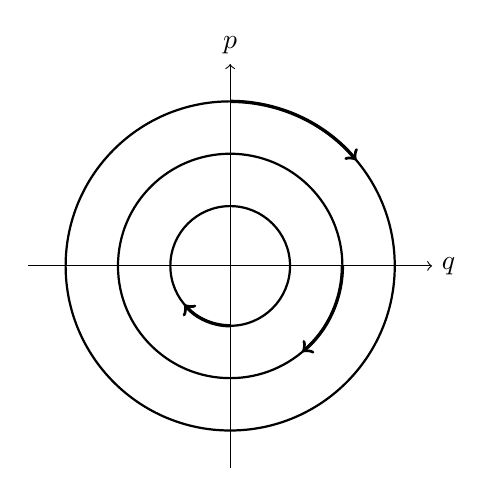
\begin{tikzpicture}[scale=0.95]
    \draw[->] (-2.7,0) -- (2.7,0) node[right] {\(q\)};
    \draw[->] (0,-2.7) -- (0,2.7) node[above] {\(p\)};
    \draw[thick] (0,0) circle (0.8);
    \draw[thick] (0,0) circle (1.5);
    \draw[thick] (0,0) circle (2.2);
    \draw[->,very thick] (0,2.2) arc[start angle=90,end angle=40,radius=2.2];
    \draw[->,very thick] (1.5,0) arc[start angle=0,end angle=-50,radius=1.5];
    \draw[->,very thick] (0,-0.8) arc[start angle=-90,end angle=-140,radius=0.8];
  \end{tikzpicture}
  \caption{La energía constante determina las circunferencias; las ecuaciones del oscilador determinan el flujo tangente en sentido horario.}
\end{figure}

\begin{classroomqa}
  \audiencequestion{¿Son las dos ecuaciones de Hamilton y \(H=E\) distintas versiones de una misma ecuación?
  \lecturetimestamp{00:15:53--00:17:06}}
  \lecturerresponse{No. Las ecuaciones de Hamilton son las dos leyes de movimiento de primer orden para un par canónico. Implican \(dH/dt=0\), de donde se deduce \(H=E\). El valor de \(E\) queda determinado por la condición inicial. La ecuación \(H=E\) identifica una superficie; por sí sola no especifica la velocidad a lo largo de ella.}
\end{classroomqa}

\section{De un estado a un flujo de estados}

En lugar de seguir una sola condición inicial, distribuyamos por el espacio de fases todas las condiciones iniciales posibles y pongamos en marcha el reloj. Cada punto representa un estado posible completo, y cada estado evoluciona según las ecuaciones de Hamilton. Podemos imaginar esa distribución como polvo o como un fluido ficticio. No se vierte ninguna sustancia en el espacio de fases: el fluido es una manera de visualizar todas las trayectorias a la vez.

El campo de velocidades en el espacio de fases es
\begin{equation}
  \mathbf V(q,p,t)
  =
  (\dot q_1,\ldots,\dot q_n,\dot p_1,\ldots,\dot p_n).
  \label{eq:l7-phase-velocity}
\end{equation}
Para un solo par canónico escribimos
\begin{equation}
  V_q=\dot q=\frac{\partial H}{\partial p},
  \qquad
  V_p=\dot p=-\frac{\partial H}{\partial q}.
  \label{eq:l7-phase-components}
\end{equation}
En cada punto, el hamiltoniano asigna un vector que indica hacia dónde se dirige a continuación el punto de fase. Si \(H\) es independiente del tiempo, el campo vectorial es estacionario: al volver al mismo punto de fase se obtiene la misma velocidad. Si \(H\) depende del tiempo, el propio campo vectorial cambia con el tiempo, pero sigue estando definido en cada instante.

\begin{figure}[htbp]
  \centering
  \includegraphics[width=0.84\textwidth]{lecture_07_figure_05.png}
  \caption{Campo de velocidades del oscilador armónico. Los vectores son tangentes a las circunferencias y se acortan al acercarse al origen.}
  \lectureframe{00:24:50}
\end{figure}

En el oscilador armónico, todos los radios giran con velocidad angular \(\omega\). Los puntos cercanos al origen tienen menor rapidez lineal porque recorren un círculo más pequeño en el mismo período. Por tanto, todo el polvo gira como un carrusel rígido.

\begin{classroomqa}
  \audiencequestion{¿Significa la rotación rígida que todas las trayectorias del oscilador tienen el mismo período?\lecturetimestamp{00:21:10--00:21:42}}
  \lecturerresponse{Sí. Esa independencia respecto de la amplitud es la propiedad especial que define al oscilador armónico. Todos los círculos se recorren con la misma frecuencia angular \(\omega\), aunque la magnitud de la velocidad en el espacio de fases sea menor en un círculo más pequeño.}
\end{classroomqa}

\begin{classroomqa}
  \audiencequestion{¿Es igual la velocidad en el espacio de fases en todos los puntos?
  \lecturetimestamp{00:24:29--00:25:37}}
  \lecturerresponse{No. Tanto su dirección como su magnitud suelen variar con la posición. En el oscilador, el vector es tangente al círculo local y tiene magnitud \(\omega\sqrt{p^2+q^2}\). Un campo vectorial asigna un vector a cada punto; no significa que se copie el mismo vector en todas partes.}
\end{classroomqa}

\begin{classroomqa}
  \audiencequestion{¿Qué son exactamente las partículas y la densidad de este fluido ficticio?\lecturetimestamp{00:56:03--00:58:40}}
  \lecturerresponse{Cada punto representa un estado completo posible del sistema mecánico entero. No representa una partícula física. Cinco partículas que se mueven en una dimensión espacial requieren cinco posiciones y cinco momentos; por tanto, el espacio de fases tiene diez dimensiones. En tres dimensiones, requiere treinta. El polvo es un conjunto de estados alternativos. Si la imagen del fluido distrae, basta con tomar una región de condiciones iniciales, hacer evolucionar todos sus puntos y comparar su volumen en el espacio de fases antes y después.}
\end{classroomqa}

\section{Compresión y divergencia}

Para preguntar si este fluido ficticio pierde volumen, empecemos en una dimensión. Supongamos que los puntos de una recta se mueven con velocidad \(v(x)\). Dos puntos próximos separados por \(\delta x\) tienen una diferencia de velocidades
\begin{equation}
  \delta v \simeq \frac{dv}{dx}\,\delta x.
  \label{eq:l7-one-dimensional-strain}
\end{equation}
Si \(dv/dx>0\), el punto delantero se mueve más rápido y el intervalo se estira. Si \(dv/dx<0\), se comprime. Por tanto, un flujo estacionario e incompresible en una dimensión satisface
\begin{equation}
  \frac{dv}{dx}=0.
  \label{eq:l7-one-dimensional-incompressible}
\end{equation}

\begin{figure}[htbp]
  \centering
  \includegraphics[width=0.84\textwidth]{lecture_07_figure_06.png}
  \caption{La construcción unidimensional que conduce a \(dv/dx\) como tasa local de estiramiento o compresión.}
  \lectureframe{00:30:20}
\end{figure}

Hay dos puntos de vista equivalentes. Podemos seguir un intervalo material y preguntar si cambia su longitud. O podemos mantener fijo un intervalo pequeño y preguntar si la cantidad que entra por unidad de tiempo es igual a la que sale. El primer punto de vista sigue el fluido; el segundo observa cómo pasa.

En más de una dimensión, una región puede estirarse a lo largo de un eje y comprimirse a lo largo de otro sin que cambie su volumen total. Para un campo de velocidades \(\mathbf V=(V_x,V_y,V_z)\), la tasa local relevante es la divergencia,
\begin{equation}
  \nabla\cdot\mathbf V
  =
  \frac{\partial V_x}{\partial x}
  +\frac{\partial V_y}{\partial y}
  +\frac{\partial V_z}{\partial z}.
  \label{eq:l7-spatial-divergence}
\end{equation}
Una divergencia positiva corresponde a expansión local; una negativa, a contracción local; y la condición de incompresibilidad es
\begin{equation}
  \nabla\cdot\mathbf V=0.
  \label{eq:l7-zero-divergence}
\end{equation}
Que el flujo de entrada y el de salida sean iguales a través de una caja pequeña fija es la misma afirmación local que la conservación del volumen de una caja pequeña que se mueve con el flujo.

\begin{figure}[htbp]
  \centering
  \includegraphics[width=0.86\textwidth]{lecture_07_figure_07.png}
  \caption{Una caja bidimensional, las componentes del flujo y la suma de las derivadas de cada componente respecto de su coordenada correspondiente, que define la divergencia.}
  \lectureframe{00:35:30}
\end{figure}

\begin{classroomqa}
  \audiencequestion{¿Hablamos de un fluido en el espacio ordinario o de un flujo en el espacio de fases? \lecturetimestamp{00:34:27--00:34:40}}
  \lecturerresponse{El argumento de la divergencia es, en primer lugar, un argumento general sobre fluidos. Lo aplicaremos al espacio de fases, de dimensión par, cuyas direcciones coordenadas son \(q_i\) y \(p_i\), y cuyas componentes de velocidad son \(\dot q_i\) y \(\dot p_i\).}
\end{classroomqa}

Volvamos ahora a los mapas discretos de estados. En un ciclo reversible, cada nodo tiene una flecha entrante y otra saliente, y una colección elegida de estados conserva el mismo número de elementos al evolucionar. En un sumidero entran muchas flechas y salen demasiado pocas; varias alternativas se vuelven indistinguibles.

\begin{figure}[htbp]
  \centering
  \includegraphics[width=0.80\textwidth]{lecture_07_figure_08.png}
  \caption{El sumidero discreto que permite relacionar de nuevo la divergencia con el criterio de la primera lección para las leyes reversibles.}
  \lectureframe{00:40:15}
\end{figure}

La pregunta continua ya está planteada con precisión: ¿tiene el flujo hamiltoniano divergencia nula, de modo que una región pequeña de estados distinguibles nunca se comprima hasta ocupar un volumen menor en el espacio de fases?

\section{Teorema de Liouville}

\begin{theorem}[Liouville's theorem]Para un sistema hamiltoniano suave, el campo canónico de velocidades en el espacio de fases tiene divergencia nula:
\begin{equation}
  \sum_i\left(
    \frac{\partial\dot q_i}{\partial q_i}
    +\frac{\partial\dot p_i}{\partial p_i}
  \right)=0.
  \label{eq:l7-liouville-divergence}
\end{equation}
De manera equivalente, la evolución hamiltoniana conserva el volumen canónico del espacio de fases
\(dq_1\cdots dq_n\,dp_1\cdots dp_n\).
\end{theorem}

\begin{classroomqa}
  \audiencequestion{¿Las componentes llamadas \(V\) son simplemente las derivadas temporales de \(p\) y \(q\)?
  \lecturetimestamp{00:42:20--00:43:22}}
  \lecturerresponse{Sí. Para un par, \(V_q=\dot q\) y \(V_p=\dot p\). Al reunir todas esas derivadas se obtiene el vector velocidad del flujo en el espacio de fases completo.}
\end{classroomqa}

Para un par canónico, las ecuaciones de Hamilton dan
\begin{equation}
  V_p=-\frac{\partial H}{\partial q},
  \qquad
  V_q=\frac{\partial H}{\partial p}.
  \label{eq:l7-liouville-components}
\end{equation}
Por tanto, la divergencia es
\begin{align}
  \frac{\partial V_p}{\partial p}
  +\frac{\partial V_q}{\partial q}
  &=
  -\frac{\partial}{\partial p}
    \left(\frac{\partial H}{\partial q}\right)
  +\frac{\partial}{\partial q}
    \left(\frac{\partial H}{\partial p}\right)\\
  &=
  -\frac{\partial^2H}{\partial p\,\partial q}
  +\frac{\partial^2H}{\partial q\,\partial p}
  =0.
  \label{eq:l7-liouville-proof}
\end{align}

\begin{figure}[htbp]
  \centering
  \includegraphics[width=0.86\textwidth]{lecture_07_figure_09.png}
  \caption{El rectángulo de diferencias finitas que permite explicar por qué las derivadas parciales mixtas de funciones suaves conmutan.}
  \lectureframe{00:47:30}
\end{figure}

La igualdad de las derivadas parciales mixtas puede verse con cuatro puntos próximos \(A,B,C,D\) en los vértices de un rectángulo pequeño del plano \(q\)-\(p\). Calcular primero una diferencia respecto de \(q\) y luego una respecto de \(p\) produce, salvo por el producto de las dos longitudes de los lados,
\begin{equation}
  F(B)+F(D)-F(A)-F(C).
  \label{eq:l7-finite-difference-combination}
\end{equation}
Calcular las diferencias en el orden inverso produce la misma combinación. En el límite de un rectángulo pequeño, esto da \(\partial_p\partial_qF=\partial_q\partial_pF\), siempre que las derivadas requeridas sean continuas.

\begin{figure}[htbp]
  \centering
  \includegraphics[width=0.88\textwidth]{lecture_07_figure_10.png}
  \caption{La divergencia canónica después de que las ecuaciones de Hamilton la han reducido a dos derivadas mixtas con signos opuestos.}
  \lectureframe{00:50:20}
\end{figure}

Para muchos grados de libertad, se produce la misma cancelación en cada par canónico:
\begin{align}
  \sum_i\left(
    \frac{\partial\dot p_i}{\partial p_i}
    +\frac{\partial\dot q_i}{\partial q_i}
  \right)
  &=
  \sum_i\left(
    -\frac{\partial^2H}{\partial p_i\,\partial q_i}
    +\frac{\partial^2H}{\partial q_i\,\partial p_i}
  \right)\\
  &=0.
  \label{eq:l7-many-pair-proof}
\end{align}
El estiramiento en una dirección canónica se compensa con la compresión en su dirección conjugada. Esta cancelación par a par expresa una estructura más profunda que una cancelación fortuita entre ejes no relacionados.

\begin{classroomqa}
  \audiencequestion{¿Se entiende que la suma se extiende a todos los pares canónicos?
  \lecturetimestamp{00:52:00--00:52:36}}
  \lecturerresponse{Sí. En la ecuación~\eqref{eq:l7-many-pair-proof} se suma sobre \(i\), y las dos derivadas mixtas se cancelan por separado dentro de cada par \(q_i,p_i\).}
\end{classroomqa}

\begin{classroomqa}
  \audiencequestion{La divergencia que se muestra parece cartesiana. ¿Se mantiene el teorema al cambiar de coordenadas?
  \lecturetimestamp{00:52:50--00:53:22,\allowbreak\ 00:58:18--00:58:40}}
  \lecturerresponse{La formulación natural se expresa en coordenadas canónicas y con el elemento de volumen canónico \(dq_1\cdots dq_n\,dp_1\cdots dp_n\). Una transformación canónica, o simpléctica, cambia a la vez las coordenadas y los momentos, y conserva ese volumen. En coordenadas no canónicas arbitrarias, la medida de volumen debe incluir un factor jacobiano; el producto ingenuo de incrementos de coordenadas puede no ser invariante.}
\end{classroomqa}

\begin{classroomqa}
  \audiencequestion{¿Requiere el teorema de Liouville un hamiltoniano independiente del tiempo? \lecturetimestamp{00:53:43--00:55:51}}
  \lecturerresponse{No. Para conservar la energía se necesitaba \(\partial H/\partial t=0\), pero en la demostración de la divergencia solo se deriva respecto de \(q_i\) y \(p_i\) manteniendo fijo el tiempo. Las derivadas parciales mixtas siguen cancelándose para \(H(q,p,t)\). Por tanto, un hamiltoniano dependiente del tiempo genera un flujo canónico dependiente del tiempo que, en cada instante, conserva el volumen.}
\end{classroomqa}

\section{Qué significa y qué no significa conservar el volumen}

Tomemos una región pequeña \(R_0\) de condiciones iniciales y hagamos evolucionar todos sus puntos durante un tiempo \(t\). El teorema de Liouville afirma que
\begin{equation}
  \operatorname{Vol}(R_t)=\operatorname{Vol}(R_0).
  \label{eq:l7-volume-preservation}
\end{equation}
La región puede desplazarse, rotar, deformarse por cizallamiento y estirarse hasta convertirse en un filamento largo. Lo que se conserva es su volumen, no su forma. En una evolución hamiltoniana suave de duración finita, distintos puntos de fase no pueden confluir en uno solo.

Para tiempos finitos, un flujo hamiltoniano suave es un mapa invertible con una inversa suave que se obtiene haciendo evolucionar el sistema hacia atrás. Esto también explica la afirmación habitual en clase de que una región conexa no puede estrangularse hasta separarse en partes desconectadas: el flujo deforma la región de manera continua y conserva su topología, aunque un cuello extremadamente delgado pueda hacer que dos lóbulos parezcan separados a resolución finita.

\begin{figure}[htbp]
  \centering
  \includegraphics[width=0.86\textwidth]{lecture_07_figure_12.png}
  \caption{Posibles deformaciones de una región del espacio de fases. Un flujo hamiltoniano suave puede formar un cuello estrecho, pero no puede dividirla realmente, en un tiempo finito, en partes que evolucionen de manera independiente.}
  \lectureframe{01:04:55}
\end{figure}

\begin{classroomqa}
  \audiencequestion{¿Puede una región del espacio de fases estrangularse y separarse en dos partes?\lecturetimestamp{01:04:10--01:05:49}}
  \lecturerresponse{No en un tiempo finito bajo un flujo hamiltoniano suave y determinista. En un hipotético punto de estrangulamiento sigue habiendo un único punto de fase con una única velocidad asignada, no dos direcciones incompatibles. La región puede desarrollar un filamento de conexión muy largo y estrecho, pero la evolución sigue siendo biunívoca y no la desgarra.}
\end{classroomqa}

\begin{classroomqa}
  \audiencequestion{¿Están físicamente conectados o entrelazados cuánticamente dos lóbulos muy separados de una región estirada?
  \lecturetimestamp{01:08:01--01:09:16}}
  \lecturerresponse{No se implica ninguna conexión física de ese tipo. La región es un conjunto de condiciones iniciales alternativas, no un objeto material. Llamarla una sola región registra el conjunto común del que evolucionaron esos estados; no dice nada sobre fuerzas ni sobre entrelazamiento cuántico entre ellos.}
\end{classroomqa}

\begin{classroomqa}
  \audiencequestion{¿Qué ocurre cerca del equilibrio inestable en posición vertical de un péndulo rígido? ¿Se solapan las trayectorias en sentido horario y antihorario?
  \lecturetimestamp{01:07:07--01:07:47}}
  \lecturerresponse{Condiciones iniciales próximas pueden separarse y seguir trayectorias muy distintas, formando los filamentos delgados que acabamos de describir. No llegan a ser el mismo punto de fase: el signo del desplazamiento infinitesimal o del momento distingue ambos lados. El estado exactamente equilibrado tiene su propio movimiento determinado de manera única: en el modelo ideal, permanece en equilibrio.}
\end{classroomqa}

\subsection{Expansión en el espacio de posiciones y contracción en el espacio de momentos}

Si una transformación canónica expande un intervalo de posiciones por un factor \(a\), la escala del momento conjugado se contrae por el factor recíproco:
\begin{equation}
  q\longrightarrow aq,
  \qquad
  p\longrightarrow \frac{p}{a},
  \qquad
  dq\,dp\longrightarrow dq\,dp.
  \label{eq:l7-canonical-scaling}
\end{equation}
Este es el contenido claro en el espacio de fases que subyace al ejemplo de la expansión de un gas. En una expansión adiabática, crece la región accesible del espacio ordinario mientras disminuyen los momentos típicos y el gas se enfría. La relación termodinámica detallada depende de la dimensión, del protocolo de expansión y de las interacciones; el teorema de Liouville impone la restricción de volumen, pero no determina todos los coeficientes termodinámicos.

\begin{classroomqa}
  \audiencequestion{¿Se aplica el mismo razonamiento a un universo en expansión, incluso si la expansión es súbita? \lecturetimestamp{00:53:23--00:56:00}}
  \lecturerresponse{El teorema de Liouville se aplica siempre que la dinámica completa sea hamiltoniana, incluso si las variables canónicas dependen explícitamente del tiempo. La expansión en las direcciones de posición debe ir acompañada de la contracción correspondiente en las direcciones del momento canónico. Sin embargo, la expansión del factor de escala cosmológico, la expansión controlada de un gas y la explosión libre de una nube no son el mismo proceso físico. Una correlación de tipo Hubble entre la distancia y la velocidad de recesión puede surgir porque los objetos más rápidos recorren distancias mayores, mientras que el enfriamiento adiabático se refiere a la contracción de la distribución local de momentos. En cualquiera de los casos, el teorema restringe el mapa completo en el espacio de fases.}
\end{classroomqa}

\begin{classroomqa}
  \audiencequestion{¿Qué utilidad práctica tiene el teorema de Liouville?
  \lecturetimestamp{01:06:16--01:07:04}}
  \lecturerresponse{Es fundamental en mecánica estadística. Determina cómo evolucionan los conjuntos de estados microscópicos y sustenta la relación entre el volumen del espacio de fases y la entropía. La expansión y el enfriamiento de un gas son una ilustración inmediata; más adelante, el teorema se convierte en una herramienta básica para razonar sobre el equilibrio y el no equilibrio.}
\end{classroomqa}

\section{Un flujo que cambia de forma drásticamente}

El oscilador armónico conserva tanto el área como la forma porque su flujo es una rotación rígida. Eso es excepcional. Para distinguir la conservación del volumen de la rigidez, consideremos
\begin{equation}
  H=\lambda pq,
  \label{eq:l7-pq-hamiltonian}
\end{equation}
donde \(\lambda\) tiene unidades de inverso del tiempo. En la clase se toma \(\lambda=1\); conservarlo permite hacer explícitas las dimensiones.

\begin{figure}[htbp]
  \centering
  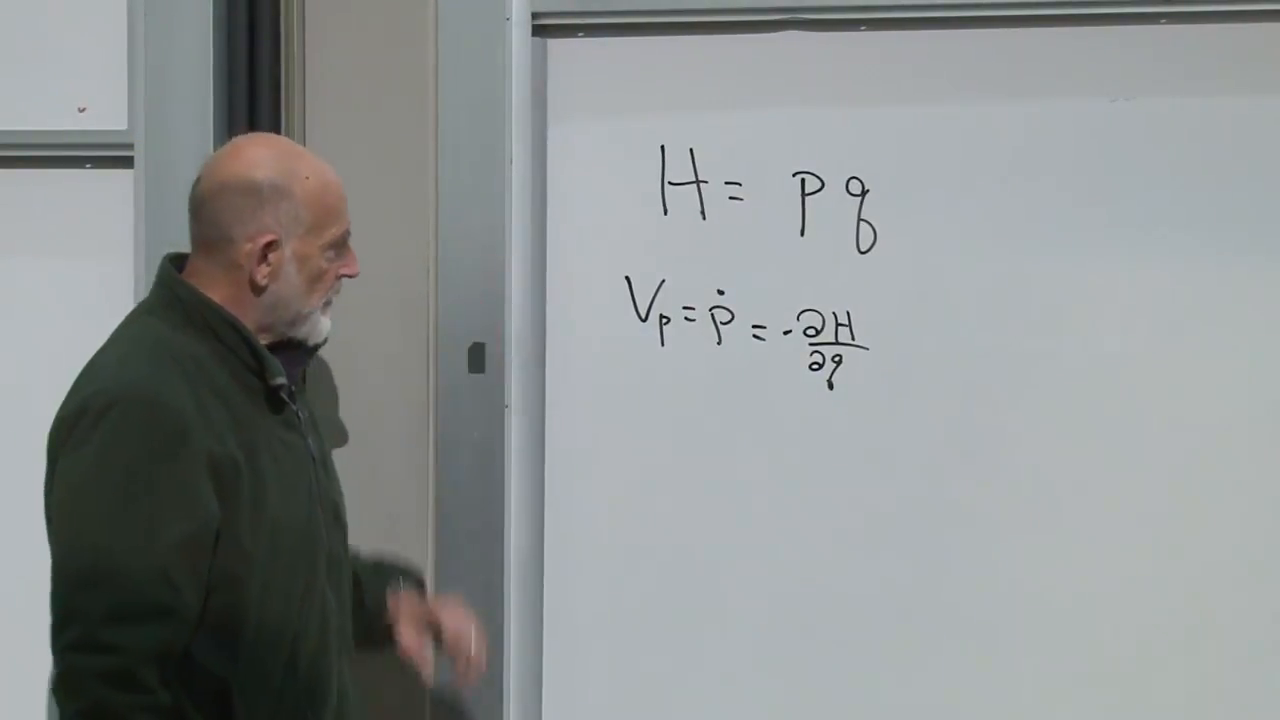
\includegraphics[width=0.82\textwidth]{lecture_07_figure_03.png}
  \caption{Comienzo del ejemplo \(H=pq\) y primera componente de la velocidad en el espacio de fases.}
  \lectureframe{01:00:11}
\end{figure}

Las ecuaciones de Hamilton son
\begin{equation}
  \dot p=-\lambda p,
  \qquad
  \dot q=\lambda q,
  \label{eq:l7-pq-flow}
\end{equation}
con soluciones
\begin{equation}
  p(t)=p_0e^{-\lambda t},
  \qquad
  q(t)=q_0e^{\lambda t}.
  \label{eq:l7-pq-solutions}
\end{equation}
Un elemento cuadrado se comprime exponencialmente en \(p\) y se estira por el mismo factor en \(q\):
\begin{equation}
  \Delta p(t)\Delta q(t)
  =
  \Delta p(0)\Delta q(0).
  \label{eq:l7-pq-area}
\end{equation}
La divergencia verifica el resultado localmente,
\begin{equation}
  \frac{\partial\dot p}{\partial p}
  +\frac{\partial\dot q}{\partial q}
  =-\lambda+\lambda=0.
  \label{eq:l7-pq-divergence}
\end{equation}

\begin{figure}[htbp]
  \centering
  \includegraphics[width=0.86\textwidth]{lecture_07_figure_11.png}
  \caption{Un parche compacto estirado hasta formar una franja larga y estrecha, con conservación del área bajo el flujo \(H=pq\).}
  \lectureframe{01:02:10}
\end{figure}

\begin{classroomqa}
  \audiencequestion{Como \(pq\) tiene unidades de acción, ¿es el teorema de Liouville una ley de conservación de la acción?\lecturetimestamp{01:03:00--01:04:09}}
  \lecturerresponse{No. El teorema conserva el volumen del espacio de fases. Para un par canónico, \(dq\,dp\) tiene unidades de acción, y ese hecho dimensional anticipa la mecánica cuántica, donde las celdas del espacio de fases se miden en unidades determinadas por \(\hbar\). Pero el producto \(pq\) no es la propia funcional de acción de Hamilton, ni es automáticamente el momento angular por el mero hecho de tener las mismas dimensiones.}
\end{classroomqa}

El ejemplo también muestra que los ángulos no tienen por qué conservarse. Una cruz con ángulo recto y componentes desiguales, sometida al escalamiento de la ec.~\eqref{eq:l7-pq-solutions}, aparece deformada por cizallamiento, aunque el área permanece invariable. El teorema de Liouville es un teorema sobre áreas o volúmenes, no sobre la rigidez euclídea ordinaria.

\section{La amortiguación produce un sumidero}

Para ver qué excluye el teorema, consideremos la ecuación reducida de un oscilador amortiguado,
\begin{equation}
  m\ddot x=-kx-c\dot x,
  \qquad c>0.
  \label{eq:l7-damped-newton}
\end{equation}
Sea \(p=m\dot x\). Entonces
\begin{equation}
  \dot x=\frac{p}{m},
  \qquad
  \dot p=-kx-\frac{c}{m}p.
  \label{eq:l7-damped-first-order}
\end{equation}
Sin amortiguación, el punto de fase gira alrededor del origen. Con amortiguación, la energía se transfiere a los grados de libertad microscópicos del medio circundante y la órbita describe una espiral hacia el interior.

\begin{figure}[htbp]
  \centering
  \includegraphics[width=0.84\textwidth]{lecture_07_figure_13.png}
  \caption{La ecuación del oscilador amortiguado y la espiral hacia el interior en el plano \(x\)-\(p\).}
  \lectureframe{01:13:30}
\end{figure}

La divergencia de este flujo bidimensional reducido es
\begin{equation}
  \frac{\partial\dot x}{\partial x}
  +\frac{\partial\dot p}{\partial p}
  =
  0-\frac{c}{m}<0.
  \label{eq:l7-damped-divergence}
\end{equation}
Todo elemento finito se contrae. El origen es un sumidero, el análogo continuo del mapa de estados en el que entran muchas flechas.

\begin{figure}[htbp]
  \centering
  \includegraphics[width=0.88\textwidth]{lecture_07_figure_14.png}
  \caption{Componentes de la velocidad en el espacio de fases del oscilador amortiguado, usadas para obtener la divergencia negativa \(-c/m\).}
  \lectureframe{01:16:05}
\end{figure}

Esto no significa que la mecánica microscópica viole el teorema de Liouville. Las dos variables \(x,p\) omiten la enorme cantidad de grados de libertad del entorno que reciben la energía del oscilador. El sistema ampliado formado por el oscilador y el entorno puede ser hamiltoniano y conservar el volumen, aunque su descripción reducida \(x,p\) se contraiga.

\begin{classroomqa}
  \audiencequestion{¿El oscilador amortiguado sigue estando descrito por la ecuación de Newton, aunque no sea hamiltoniano en este espacio de fases reducido?
  \lecturetimestamp{01:20:09--01:21:12}}
  \lecturerresponse{Sí. La ecuación \(F=ma\) puede incluir una fuerza de arrastre determinada empíricamente. La descripción elemental mediante \(L=T-V\) y el formalismo hamiltoniano se aplica directamente a fuerzas conservativas; los lagrangianos más generales también permiten tratar algunas fuerzas que dependen de la velocidad. Sin embargo, un término de fricción markoviano para un par aislado \(x,p\) describe una dinámica disipativa reducida, no un sistema hamiltoniano canónico cerrado.}
\end{classroomqa}

\begin{classroomqa}
  \audiencequestion{Si las ecuaciones del movimiento amortiguado pueden integrarse hacia atrás con precisión infinita, ¿se pierde realmente información?
  \lecturetimestamp{01:25:16--01:27:17}}
  \lecturerresponse{Para cualquier tiempo finito, la ecuación diferencial ideal sigue teniendo una inversa, de modo que los datos exactos pueden evolucionar hacia atrás. La afirmación precisa es que las celdas finitas del espacio de fases se contraen exponencialmente. Recuperar entonces su estado pasado requiere una precisión que aumenta exponencialmente y, en el límite de tiempo infinito, todas las trayectorias se aproximan al sumidero. Esta es la analogía clásica continua más cercana a la imagen discreta de pérdida de alternativas; no afirma que dos soluciones exactas a tiempo finito se conviertan literalmente en una sola.}
\end{classroomqa}

\begin{classroomqa}
  \audiencequestion{¿Puede un campo vectorial tener divergencia nula sin proceder de un sistema hamiltoniano? \lecturetimestamp{01:18:21--01:22:34}}
  \lecturerresponse{Desde luego. La forma hamiltoniana es suficiente para que la divergencia sea nula, pero no es necesaria. Un campo de velocidades incompresible arbitrario puede tener divergencia nula sin ser un campo hamiltoniano canónico en ese mismo espacio. El campo de velocidades de un fluido incompresible tridimensional es el ejemplo habitual en clase: tres coordenadas no pueden formar por sí solas pares canónicos. La mecánica completa de fluidos puede admitir formulaciones hamiltonianas más elaboradas e infinito-dimensionales, pero eso no invierte la implicación unidireccional que se establece aquí.}
\end{classroomqa}

\section{Otras distinciones que ponen de manifiesto las preguntas}

\begin{classroomqa}
  \audiencequestion{¿Qué relación hay entre el movimiento sobre una superficie de energía constante y la conservación de todo un volumen del espacio de fases?
  \lecturetimestamp{01:28:47--01:30:41}}
  \lecturerresponse{Son consecuencias independientes de la estructura hamiltoniana. Si \(H\) no depende del tiempo, cada trayectoria permanece en su propia superficie de energía. Una región finita puede atravesar muchas de esas superficies; el teorema de Liouville afirma que se conserva el volumen de toda esa región. En el oscilador armónico, la región también conserva su forma porque el flujo es una rotación rígida. La región \(H=pq\) conserva solo su área, no su forma.}
\end{classroomqa}

\begin{classroomqa}
  \audiencequestion{¿Qué lugar ocupa el trabajo mecánico en la descripción hamiltoniana?
  \lecturetimestamp{01:30:44--01:32:57}}
  \lecturerresponse{El trabajo describe la energía transferida a través de la frontera elegida para un sistema. Un agente externo puede elevar un peso o cambiar un parámetro y, con ello, modificar la energía del subsistema; el agente pierde la energía que suministra. Si se incluyen ambos lados en un único modelo cerrado, el énfasis vuelve a la conservación de la energía total y al intercambio entre subsistemas.}
\end{classroomqa}

\begin{classroomqa}
  \audiencequestion{¿La conservación del volumen conserva también la topología y los ángulos?
  \lecturetimestamp{01:33:00--01:33:37}}
  \lecturerresponse{Un flujo hamiltoniano suave a tiempo finito conserva la topología porque es una deformación continua e invertible. En general, no conserva los ángulos ni la forma euclidianos. La rotación rígida del oscilador sí lo hace, pero el estiramiento \(H=pq\) muestra que se trata de un caso especial.}
\end{classroomqa}

\begin{classroomqa}
  \audiencequestion{¿Se omitió la transformación de Legendre porque carece de significado físico?
  \lecturetimestamp{01:33:43--01:34:48}}
  \lecturerresponse{No. Es una transformación útil que intercambia la descripción en términos de velocidad por la descripción en términos de momento y da lugar a \(H=\sum_i p_i\dot q_i-L\) cuando la aplicación es regular. Ya se ha recurrido repetidamente a esta construcción, aunque no se destacara su nombre formal; para el teorema que nos ocupa no hace falta desarrollar la teoría general en detalle.}
\end{classroomqa}

\section{Corchetes de Poisson: la siguiente reducción}

Los últimos minutos retoman el tema histórico. La mecánica del siglo XIX buscó repetidamente estructuras compactas que relacionaran sistemas aparentemente distintos---la mecánica y la óptica geométrica, las partículas y los rayos, las trayectorias clásicas y las descripciones ondulatorias. Los corchetes de Poisson son otra estructura de este tipo y adquieren especial importancia en la mecánica cuántica.

Sea \(F(q,p)\) una función cualquiera del espacio de fases. Podría ser una coordenada, un momento, el producto \(qp\) o el momento angular. A lo largo del movimiento,
\begin{equation}
  \frac{dF}{dt}
  =
  \sum_i\left(
    \frac{\partial F}{\partial q_i}\dot q_i
    +\frac{\partial F}{\partial p_i}\dot p_i
  \right).
  \label{eq:l7-f-time-derivative}
\end{equation}
Sustituyamos las ecuaciones de Hamilton:
\begin{equation}
  \frac{dF}{dt}
  =
  \sum_i\left(
    \frac{\partial F}{\partial q_i}
    \frac{\partial H}{\partial p_i}
    -
    \frac{\partial F}{\partial p_i}
    \frac{\partial H}{\partial q_i}
  \right).
  \label{eq:l7-f-hamiltonian-derivative}
\end{equation}

\begin{figure}[htbp]
  \centering
  \includegraphics[width=0.88\textwidth]{lecture_07_figure_15.png}
  \caption{La regla de la cadena para la derivada temporal de una función general del espacio de fases, \(F(q,p)\).}
  \lectureframe{01:42:40}
\end{figure}

La combinación antisimétrica que se repite merece un nombre. Para dos funciones cualesquiera, \(F\) y \(G\), definimos su corchete de Poisson como
\begin{equation}
  \boxed{
  \{F,G\}
  =
  \sum_i\left(
    \frac{\partial F}{\partial q_i}
    \frac{\partial G}{\partial p_i}
    -
    \frac{\partial F}{\partial p_i}
    \frac{\partial G}{\partial q_i}
  \right).}
  \label{eq:l7-poisson-bracket}
\end{equation}

\begin{figure}[htbp]
  \centering
  \includegraphics[width=0.86\textwidth]{lecture_07_figure_16.png}
  \caption{La combinación de derivadas de dos funciones, al convertirse en el corchete de Poisson.}
  \lectureframe{01:44:15}
\end{figure}

La ecuación~\eqref{eq:l7-f-hamiltonian-derivative} se convierte en
\begin{equation}
  \boxed{\frac{dF}{dt}=\{F,H\}.}
  \label{eq:l7-hamiltonian-poisson-evolution}
\end{equation}
Si \(F\) también depende explícitamente del tiempo, se añade \(\partial F/\partial t\). Al tomar \(F=q_i\) o \(F=p_i\) se recuperan las dos ecuaciones de Hamilton, de modo que la ecuación~\eqref{eq:l7-hamiltonian-poisson-evolution} es una forma compacta de expresar la dinámica completa.

La notación siempre puede comprimirse de manera artificial---se podrían elevar al cuadrado muchas ecuaciones, sumarlas y llamar ecuación al resultado. Eso ocultaría la estructura en vez de revelarla. El corchete de Poisson es útil precisamente por la razón opuesta: su álgebra organiza la evolución temporal, las cantidades conservadas y la simetría. El siguiente paso es desarrollar esa álgebra y aplicarla al momento angular, cuya estructura será fundamental tanto en la mecánica clásica como en la teoría cuántica.

\section{El significado continuo de la reversibilidad}

Ya podemos exponer la cadena de ideas sin abreviarla. Las ecuaciones de Hamilton conservan \(H\) cuando el hamiltoniano no depende explícitamente del tiempo, por lo que las trayectorias individuales permanecen en hipersuperficies de energía constante. Esas mismas ecuaciones asignan una velocidad a cada punto del espacio de fases. La divergencia de ese campo de velocidades se anula porque las derivadas parciales mixtas se cancelan por pares. En consecuencia, una región entera de estados posibles conserva su volumen canónico.

Esta es la versión continua de una flecha de entrada y una de salida. La forma y los ángulos pueden cambiar, y las trayectorias vecinas pueden separarse enormemente. Lo que no puede ocurrir en una descripción hamiltoniana cerrada y suave es que un conjunto finito de alternativas se comprima hasta ocupar un volumen menor del espacio de fases. El flujo \(H=pq\) muestra la posibilidad de estiramiento; el oscilador amortiguado reducido muestra el sumidero que aparece cuando se abandonan las condiciones hamiltonianas. Los corchetes de Poisson condensan entonces la misma dinámica en la afirmación de que el hamiltoniano genera cada derivada temporal.
